
\documentclass[letterpaper, 10 pt, conference]{ieeeconf}  % Comment this line out if you need a4paper

%\documentclass[a4paper, 10pt, conference]{ieeeconf}      % Use this line for a4 paper

\IEEEoverridecommandlockouts                              % This command is only needed if 
                                                          % you want to use the \thanks command

%\usepackage{bibtex}
%\addbibresource{icra.bib}

\overrideIEEEmargins                                      % Needed to meet printer requirements.

% See the \addtolength command later in the file to balance the column lengths
% on the last page of the document

% The following packages can be found on http:\\www.ctan.org
%\usepackage{graphics} % for pdf, bitmapped graphics files
%\usepackage{epsfig} % for postscript graphics files
%\usepackage{mathptmx} % assumes new font selection scheme installed
%\usepackage{times} % assumes new font selection scheme installed
%\usepackage{amsmath} % assumes amsmath package installed
%\usepackage{amssymb}  % assumes amsmath package installed
\usepackage{graphicx}
\usepackage{url}
\title{\LARGE \bf
Evaluating Impact in the ROS Ecosystem
}


\author{William Curran$^{1}$, Thomas Thornton$^{2}$, Benjamin Arvey$^{1}$, and William D. Smart$^{1}$ % <-this % stops a space
\thanks{$^{1}$William Curran, Benjamin Arvey and William D. Smart are with the Department of Mechanical, Industrial and Manufacturing Engineering, Oregon State University, Corvallis, Oregon.
        {\tt\small curranw@onid.orst.edu, arveyb@onid.orst.edu, bill.smart@oregonstate.edu}}%
\thanks{$^{2}$Thomas Thornton with the Department of Computer Science, Colby College, Waterville, Maine.
        {\tt\small twthornt@colby.edu}}%
}


\begin{document}



\maketitle
\thispagestyle{empty}
\pagestyle{empty}


%%%%%%%%%%%%%%%%%%%%%%%%%%%%%%%%%%%%%%%%%%%%%%%%%%%%%%%%%%%%%%%%%%%%%%%%%%%%%%%%
\begin{abstract}
The ROS ecosystem is an interconnected web of packages, nodes and people with no efficient means to compare, assess or visualize them. We develop a set of tools consisting of various metrics, a data visualization web app, and an active monitoring system. With these tools, we measure the current state of the ecosystem as well as determine where the community should direct their efforts. We also encourage the community to provide input on potential applications, additional metrics, and further improvements to address the needs of the ROS ecosystem. We incentivize this input by gamifying community contributions to the infrastructure. Encouraging user-driven improvements to the ROS infrastructure through the use of a leaderboard and friendly competition will advance ROS development and community support far into the future.

\end{abstract}


%%%%%%%%%%%%%%%%%%%%%%%%%%%%%%%%%%%%%%%%%%%%%%%%%%%%%%%%%%%%%%%%%%%%%%%%%%%%%%%%
\section{INTRODUCTION}

The Robot Operating System (ROS) is a set of software libraries and tools that help roboticists build robot applications. Writing software for robots is difficult because there are many types of robots with wildly varying hardware. ROS reduces this difficulty by providing a general and structured communication layer above the driver level. ROS has become the standard multi-platform robot operating system and the popularity of ROS has risen over the years with 3,570,374 downloads during July 2014 alone \cite{ros-metrics}.

As ROS becomes larger, the greatest challenge for the community is understanding how end-users use ROS and where to focus the efforts of community members. In this work, we built three tools that give us a more accurate picture of what's going on in the ecosystem. These tools allow us to: 

\begin{enumerate}
\item Collect usage information to form an accurate and dynamic picture of how nodes and packages are used.
\item Measure the impact and health of a particular package, node, or contributor.
\item Visualize this information graphically with an interactive, web-based interface
\end{enumerate}
Used together, these tools provide the information we need to understand how the ROS development community can best direct its efforts.

We have developed a set of metrics for ROS nodes, packages, and people, which is roughly analogous to citation counts and h-indices in traditional academic publishing. The metrics are based on a dependency analysis, and include data gathered from GitHub, the Wiki, and answers.ros.org. Knowing which code has the most impact on the end-user community will help us better focus development effort, prioritize resources, and encourage contributions.

We have also developed an instrumented version of roscore that allows live usage statistics on nodes and communications to be recorded, saved to disk, and sent back to an aggregating server at Oregon State University. The system is designed to be lightweight, transparent, and completely opt-in.  Users can choose not to record anything, only to record locally, or to send anonymous information back for aggregation. Actual usage statistics allow us to determine how many people use ROS or how many people run the nav stack under ROS Hydro more accurately. We can see which nodes end-users use in installations, and begin to get an empirical measure of reliability (a node that is used a lot and that has few open tickets is probably reliable).

Finally, we have developed a highly-customizable, web-based visualization tool to show this dependency and impact information at an adjustable level of detail. This allows us to present the data in a more readily understandable, interactive form that will allow users to explore the relationships among nodes, packages, and people to identify and isolate trends.

The remainder of this paper is organized as follows. Section 2 describes the current state of Robot Operating System, and the motivation behind open source development. Section 3 describes our live usage statistics monitor, ROSKomodo, and the metrics it uses. Section 4 describes our static analysis of GitHub repositories and the ROS Wiki to develop static metrics of impact and health. Section 5 demonstrates how this data can easily be graphed with our custom web-based interface. Section 6 demonstrates how the metrics and tools developed in this work should be used to gamify ROS development, followed by our conclusion in Section 7.
\section{Background}

To motivate this work, we briefly outline ROS and give an overview of its current state. We also analyze related work in the motivational factors behind open source development. Throughout this work we utilize these motivational factors to make design decisions for the tools we develop. 

\subsection{Robot Operating System}
Robot Operating System (ROS) \cite{288} is a collection of packages that provides an abstract and fast framework for robot software development. Traditionally, software development in robotics had been entirely custom-made for each robot, slowing research and development. Quigley et al. \cite{288} developed ROS to avoid this problem by using a generic communication infrastructure between high-level and low-level hardware, essentially abstracting away the hardware layer and allowing users to use the same code on many different robots. 

ROS has a directed graph architecture, where edges represent messages and nodes represent processes. Nodes perform computation and communicate with each other by passing strictly-typed data structures called messages. Low-level hardware nodes either publish messages, such as laser scanner data, or subscribe to messages, such as motor controls. A roboticist typically builds a high-level node in ROS by subscribing to messages published by low-level hardware nodes, performing some computation, and publishing its own message, which is in turn subscribed to by another node. This makes ROS highly modular and abstract, promoting encapsulation and code reuse.

The current state of ROS is healthy. The open-source community contributes hundreds of commits every day to a variety of new packages \cite{ros-metrics}. However, ROS is a few years old, and many of the original maintainers of the core packages of ROS have moved on, or are overloaded with maintaining many other packages. ROS is growing, and is beginning to suffer from having too few people maintaining too many packages. The top 10 maintainers of ROS maintain 33\% of the 1500 currently supported packages. This means many reported issues remain unresolved. For example, one of the core packages in ROS, $ros\_comm$, has 104 open issues. Many of these issues have been open for months, as maintainers focused efforts on more critical issues. Ideally, important packages should have issues resolved quickly.

ROS has a modular structure, meaning each node depends on the flawless execution of many other nodes. If some of those nodes have many open issues, or no longer recieve support, a new node that depends on them may also have issues. It is important to prevent bugs from propagating through the system, but it can be difficult to find the node from which each bug originates. 

In this work, we develop a health metric and an impact metric for each node based on live usage statistics and a static analysis. The health metric informs the community about which nodes are unsupported, or have many issues to resolve. The impact metric describes which nodes have the most impact on other nodes. With these metrics combined, the community can find where to focus their effort when supporting ROS.

\subsection{Motivation for Open Source Development}

To understand the motivating factors behind community support of ROS, we need to first understand the motivation behind the community support of open source software in general. Krogh et al. has categorized these into intrinsic, internalized extrinsic and extrinsic motivations \cite{VonKrogh:2012:CRM:2481639.2481654}. An open-source developer is extrinsically motivated when they work to obtain some separable outcome, and is intrinsically motivated when they develop for interest or pleasure \cite{Deci_Motivation}. In this section we discuss these motivating factors, and how to apply them to our work.

We mainly focus on intrinsic and internalized extrinsic motivations. Internalized extrinsic motivations are extrinsic, but could be internalized. These are perceived as self-regulating behavior rather than external motivations \cite{Roberts:2006:UMP:1246148.1246151}. Internal motivations can be linked to internalized extrinsic motivations. For example, Lakhani and von Hippel \cite{Lakhani00howopen} linked feelings of competence and fun to willingness to help other developers. Since ROS is entirely community-built, developing tools to make ROS a more enjoyable and fun experience encourages community assistance. Lakhani and von Hippel also note that individuals are motivated by reciprocal helping behavior. If we include tools to help increase feelings of competence and fun, that will increase the community willingness to help other developers. This in turn motivates those developers to reciprocate.

Peer reputation is also a powerful motivational tool. A variety of surveys report that peer reputation is a large driving factor for participation in the community \cite{ghosh_understanding_2005, 927045, 33992}. Without significant effort from a developer to contribute to the community through Q\&A forums and mailing lists, there is little opportunity for community reputation based purely on code quality and impact.

\section{Live Usage Metrics}

To help develop an accurate picture of how end-users use nodes, we developed ROSKomodo, an instrumented version of $roscore$ that monitors and aggregates live usage statistics. This version of $roscore$ is lightweight, transparent, opt-in and non-invasive. We will first give an overview of ROSKomodo and the related privacy concerns. We then describe the implementation and the aggregated live usage metrics. 

\subsection{Overview}

Live usage metrics will answer many questions that cannot be answered by the current infrastructure. Being able to discover how many people are using ROS, or how many users are upgrading to the newest ROS distributions will greatly assist in discovering where to focus the support and effort of the community.

We cannot fully understand the impact of a specific node in ROS without understanding which nodes end-users regularly use. The current infrastructure derives this metric from an aggregation of the number of downloads per package \cite{ros-metrics}. This is highly inaccurate. ROSKomodo, combined with a static analysis (Section 4) gives us clear understanding of which nodes are the most depended on and used by end-users.

Lastly, the operating system, operating system distribution and ROS distribution all play a large factor in ROS running smoothly. If many users are not upgrading to a new ROS distribution due to specific concerns, or many users use an unsupported operating system distribution, the maintainers need the tools to detect this and re-analyze what the community wants as a whole.

\subsection{Privacy}

It is important to understand the privacy concerns of the ROS community. ROSKomodo is entirely opt-in and non-invasive, with a variable level of reporting. We built ROSKomodo as a stand-alone ROS package that can be easily added to, or removed from, the $roscore$. By querying the community, we found that users want ROSKomodo to include varying levels of opt-in. This is crucial for user participation. Many users in industry have proprietary software and do not wish to disclose any usage information, and many users have personal issues with disclosing geographical information about themselves. However, without the contribution of the community, these tools will be ineffective. Making it opt-in alleviates many of the privacy concerns of the community.

One of our biggest concerns was how to install ROSKomodo on the user's machine. The installation can be built into $roscore$ and ask the user to opt-in, or the user can inherently opt-in by choosing to download the package manually. By adding the package to the core of ROS, we would have more user contribution, but must be completely transparent. On the other hand, if the users must manually install ROSKomodo, the user contribution would decrease, but transparency would be less of an issue. We decided to implement a modified version of roscore, and the users will be given the choice to opt-in the first time, and only the first time, they execute ROS. This will expose more of the community to ROSKomodo, and still retains complete transparency.

Varying opt-in levels will allow users to choose the level of privacy they wish. Currently we have three levels of opt-in, but are open to adding additional levels based on community response. The user can report:

\begin{enumerate}
\item Usage, environment information and personal information.
\item Usage and environment information.
\item Usage information
\end{enumerate}
The user can also choose whether they would like to autonomously send information to the database, or to manually send it to our databases using a packaged script. The local XML file contains all of the information that we send to our servers. The user can read these files and decide at a later time if they would like to opt-in. This level of transparency addresses many privacy concerns, and should encourage more users to report their live usage statistics. 


\subsection{Implementation}

We implement ROSKomodo in two parts: logging and reporting. The logging is meant to be included in every distribution of ROS, because it can be useful for other applications, and the reporting is entirely opt-in.

Whenever a user launches a node in ROS, a Python logger is created to keep track of the environment, node information, and communication between nodes. These are all compiled together and output in a logging file to be used for debugging purposes. This already exists within the ROS infrastructure. We intercept these logs as they are created, wrap the pertinent metrics into a ROSKomodo topic, and publish it. We built the ROSKomodo logging infrastructure with extendability in mind. If we wish to log additional metrics, we may add those metrics to the existing Python logging infrastructure.

This information is also useful for debugging purposes. A user can subscribe to published ROSKomodo messages and detect when nodes are launching, when topics are starting or stopping, and when nodes shut down.

The ROSKomodo reporting system subscribes to the ROSKomodo logging topics, aggregates the statistics based on the users opt-in level, and reports the statistics to our database and a local XML file. ROSKomodo reporting is where a user can choose their level of opt-in, and is the core of our online metric reporting system.

\subsection{Live Usage Metrics}

We record live usage metrics associated with topics and nodes. For topics, we record the topic name, the topic type (publisher/subscriber), the topic data structure, and the duration of connection. Using this information, we are able to discover which nodes depend on the published topics of other nodes. For example, to perform localization, the localization node subscribes to a map, which is in turn published by a mapping node. We cannot discover this dependency through static analysis, and node maintainers must add this information manually to the online documentation. The automation of this process would be useful to the ROS community.

For nodes, we record the node name, the package that node belongs to, the operating system, IP address, MAC address, ROS distribution, duration, and whether the code is running on the robot, or on a server connected to the robot. Since ROS has a server-like architecture, a user could use ROS in Windows to publish commands to a robot in Linux. If many people are doing this, maybe the maintainers should fully support both operating systems. These are the solutions ROSKomodo is built to help maintainers develop. We also include the IP address to find which robots researchers use in a specific geographical location, and the MAC address to find a concrete answer to how many computers have ROS installed.

ROSKomodo easily obtains these informative live usage metrics. Over the next year we will ask the community whether they would like additional metrics, or if they would prefer us to remove some. Community feedback is important when deciding if ROSKomodo is obtaining both useful and informative metrics while respecting privacy concerns. 


\section{Static Analysis of the ROS Ecosystem}

The ROS ecosystem spreads across different environments and takes different forms. The Wiki contains package listings, tutorials, and other documentation. GitHub hosts package repositories and provides a platform for collaboration. The package manifests document explicit dependencies. All of these entities are connected through ROS. The data these resources hold is necessary to elucidate the current state of the ecosystem and to construct accurate and meaningful metrics.

\subsection{External Information Aggregation System}
We have created an information aggregation system to accomplish this goal. The process starts with the current ROS distribution file, which lists the available packages and their associated repositories. Repository information is obtained from GitHub, including issues, involved users, and more. Finally, the manifest files are extracted from the repositories, which hold package-specific information, along with the names of key persons (authors, maintainers, GitHub users).

The information collected is subsequently combined to create composite metrics for impact, health, activity, and more. Package impact is derived from the dependency network. Packages that are depended on directly or indirectly (discounted by degrees of separation) by many others receive a high impact score. We propagate the impact of a package to its maintainers and authors to create the metric for contributor impact. We derive package health from the number of maintainers and the types of maintainers (based on email). The combination of this metric with the live usage statistics accurately reflects package health. We calculate repository health from the number and recency of issues and the associated labels, along with the number of days since the last update, repository size and owner type (Table \ref{HealthGithub}). We then combine package health with repository health to form a composite metric. Lastly, we calculate GitHub user activity from the number of issues opened by and assigned to a user. With available user emails, this metric is linked to package maintainers and authors to create a metric of contributor impact. All of these composite metrics are controlled through a series of weight configuration files. This allows us to easily adjust the weights, both for our own experimentation and to better fit the priorities of the ROS community.

\begin{table}
\centering
\begin{tabular}{|l|c|l|}
\hline
Name & Value & Description \\
\hline
Subscribers & 0.25 & Number of subscribers \\
\hline
Watchers & 0.55 & Number of watchers \\
\hline
Updated At & -0.15 & Number of days since last update \\
\hline
Repo Size & -0.02 & Number of kilobytes \\
\hline
Owner Type & 0.5 & Is an organization (not an individual) \\
\hline
Closed Issue & .015 & If an issue is closed \\
\hline
Assigned Issue & .5 & If an issue is open and assigned \\
\hline
Created At & -.25 & Number of days since issue was opened \\ 
\hline
Bug & -0.5 & If an issue is labeled a bug \\
\hline
Enhancement & 0.5 & If an issue is labeled an enhancement \\
\hline
Critical & -0.95 & If an issue is labeled critical \\
\hline
Major & -0.75 & If an issue is labeled major \\
\hline
Minor & 0.25 & If an issue is labeled minor \\
\hline
\end{tabular}
\caption{Repository health (estimated need of maintenance) is calculated from this list of values. The overall package health is a combination of repository health and ROS package health.}
\label{HealthGithub}
\end{table}

\subsection{Community Relevance}

Aggregating multi-source information about the ecosystem holds several benefits for ROS. We are now able to efficiently and accurately discover the current state of the ecosystem. For example, we have eaisly found that 837 packages have a BSD license, 930 different GitHub users have opened an issue on a ROS repository, and $roscpp$ is the most commonly run package. Over time, these numbers will change, but the information will be stored. We can observe statistics such as the ratio of maintainers to packages, or the average repository's number of days since the last update. These and others can help reveal how the ecosystem is changing over time and what trends it follows. 

The metrics derived from the accumulated information are especially relevant to the community members of ROS. Metrics like impact provide tangible feedback to contributors. This calls attention to the efforts of those who excel at package maintenance, and motivates others. This adds a degree of gamification and might hold some of the associated benefits (increasing user engagement, activity level, and collaboration). Maintainers can also use composite metrics like health to assess and improve community initiatives. This provides useful information to adjust the strategies and approaches of these initiatives. In the future development, we can adjust these metrics, and new metrics could be added, depending on the desires of the community.

Using our static metrics, we analyzed the health of the top 10 impactful nodes in ROS (Table \ref{ImpactHealthTable}). Two nodes stand out as having high impact and low health: $roscpp$ and $rospy$. Both nodes exist within the same GitHub repository, causing an identical health metric. This repository, $ros\_comm$ is a core ROS package that almost every node depends on. It currently has 104 open issues with 29 bugs, 54 enhancement requests, and 21 unlabeled issues. Using these static metrics can report to the community where to focus bug fixes.

\begin{table}
\centering
\begin{tabular}{|l|c|c|}
\hline
Node Name & Impact & Health \\
\hline
catkin & 1 & .565489 \\
\hline
std\_msgs & .488538 & .634868 \\
\hline
roscpp & .486213 & .201382 \\
\hline
message\_generation & .444518 & .629212 \\
\hline
message\_runtime & .439037 & .632097\\
\hline
rospy & .35515 & .201382 \\
\hline
geometry\_msgs & .322093 & .626917 \\
\hline
rostime & .304817 & .6341 \\
\hline
roscpp\_serialization & .292691 & .6341 \\
\hline
cpp\_common & .29186 & .6341 \\
\hline
\end{tabular}
\caption{By analyzing impact (the amount that node is depended on) and health (a combination of repository and ROS package health), we can easily isolate issues with core ROS packages and report these issues to the community.}
\label{ImpactHealthTable}
\end{table}

\section{Visualization of Metrics}

\begin{figure*}[th!]
\centering
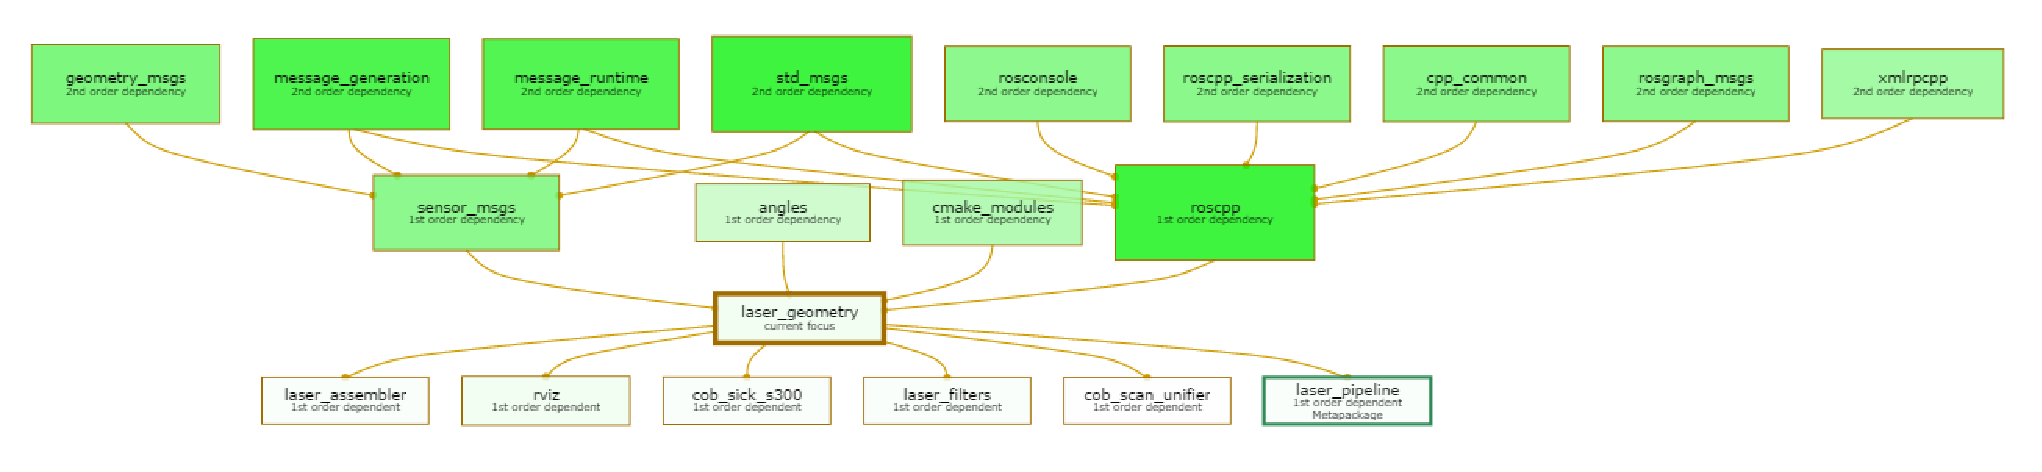
\includegraphics[width=2.0\columnwidth]{laser_geo}
\caption{The first two orders of dependencies, and one order of dependents for the laser\_geometry node. The shade of color represents the impact of that node, with the darker nodes having higher impact. Note that laser\_geometry depends on a total of 49 nodes, and as depended on by 82 nodes.}
\label{laser_geo_vis}
\end{figure*}


In order to make the metrics and analysis more accessible, we develop a web visualization based on the dependency structure of nodes, a directed acyclic graph \cite{ros-komodo-vis}. We built our visualization on the XTrace API \cite{xtrace}. Package nodes are represented by rectangles, where users can configure color and size to display different data sets. Dependencies form the edges of the graph, and are represented by spline curves with dots on the dependent node.

One major advantage of the visualization is its utility for tracing dependencies. In ROS, many different people contribute to the infrastructure. For example, many people do not develop the navigation stack, but many people use it. It is useful to know if a node depends on an unsupported part of the navigation stack. Determining first order dependencies of a given node is a simple task, but finding dependencies separated by more than one degree is much more daunting. This visualization assists the user in finding if a node depends on an unsupported node many degrees of separation away.

Another important feature of the visualization reduces the scope of the current view in order to identify and isolate trends in the metrics that may not be apparent from leaderboards or tables alone (Figure \ref{laser_geo_vis}). Given that current ROS distributions have over a thousand packages, it is necessary to reduce the graph to specific areas of interest. The user chooses a node to focus on and sets the number of degrees to show, and all other nodes are hidden. Transitive reduction is also useful in making sense of otherwise crowded systems. Lastly, the user can manually hide and show nodes to customize the view.

The visualization is also designed to enable users to explore the relationships among nodes and people. Users can create and share views of the ecosystem by generating and sending a link to their current graph settings. Impact and health metrics are represented in the visualization as node colors, and color scales are customizable (Figure \ref{laser_geo_vis}). For instance, the visualization can display a metric as a heatmap, a rainbow, or a shade of a single color (as shown above).

\section{Gamification}

Open-Source users must intrinsically desire to improve or create needed ROS packages. One of the methods to catalyze this process that has been identified is gamification \cite{hamari_gamification}. Currently, after publishing a software package on ROS, or fixing an existing one, the contributor receives little reinforcement for this behavior. If the roboticists using ROS could view a quantity denoting the impact of their software package displayed amidst other users' scores (essentially, a leaderboard), this would provide motivating feedback to improve the ROS ecosystem

Gamification, directly and indirectly related to software development, has yielded positive results in many studies \cite{Dubois:2013:UGM:2491411.2494589,Ahmed-Game,hamari_gamification,Li-Engaging}. It increases user engagement, activity level, and collaboration. The qualities elicited by gamification could be immensely beneficial to the ROS ecosystem. The studies above created completely gamified environments with badges, challenges, level systems and more. Rather than developing all of these features at once for ROS, the single, highly effective component of a leaderboard \cite{Ahmed-Game} will be introduced.

Much of the work necessary to developing a leaderboard is outside the scope of any previous study or paper on gamification. The software infrastructure of ROS is unique and such a strategy of quantifying package importance has not been attempted by the community. Once this metric is developed, the related works about gamification and leaderboards will be useful for the front-end implementation.

A leaderboard will be effective for two reasons. First, it will introduce an element of competition to ROS. This has been shown to increase the effects of gamification \cite{Dubois:2013:UGM:2491411.2494589}, principally, user engagement. Contributors may see where their packages rank in relation to others. This introduces the social aspect that has been shown to positively affect user activity in gamification studies \cite{Li-Engaging}. A leaderboard could either motivate a contributor to create a package that will be ranked higher (meaning it is more important/impactful), or it will provide positive feedback for a user who has created a package that is ranked highly.

\section{Conclusion}

Throughout this work, we have grounded our development on the motivational factors behind open-source development. Gamification is used to catalyze intrinsic motivations, such as fun, and has been linked to a willingness to help other developers. The ROS node health and impact metrics we developed (Sections 3 and 4) directly assist the creation of leaderboards and friendly competition.

This friendly competition is directly linked to peer reputation. As mentioned earlier, peer reputation is a driving factor for participation in the community. With every competition, there must be a small number of top performing developers. By placing these names on the front page of the ROS Wiki, these individuals will be publicly recognized and will personally benefit from a greater reputation. The metrics and tools we have developed in this work directly contribute to the creation of these leaderboards.

These tools also let us perform interesting analyses of the social network of ROS contributors. We can analyze how many collaborations exist across organizational or geographic boundaries, how many packages are authored and maintained by people in the same organization, how many of the ROS-Industrial packages are depended on non ROS-Industrial packages, or what is a contributors Quigley Number? While these analyses do not directly address current issues in the ecosystem, they do provide high-level insight into how ROS is being used, and this will help us figure out how we should grow as a community.

\addtolength{\textheight}{-12cm}   % This command serves to balance the column lengths
                                  % on the last page of the document manually. It shortens
                                  % the textheight of the last page by a suitable amount.
                                  % This command does not take effect until the next page
                                  % so it should come on the page before the last. Make
                                  % sure that you do not shorten the textheight too much.

%%%%%%%%%%%%%%%%%%%%%%%%%%%%%%%%%%%%%%%%%%%%%%%%%%%%%%%%%%%%%%%%%%%%%%%%%%%%%%%%



%%%%%%%%%%%%%%%%%%%%%%%%%%%%%%%%%%%%%%%%%%%%%%%%%%%%%%%%%%%%%%%%%%%%%%%%%%%%%%%%



%%%%%%%%%%%%%%%%%%%%%%%%%%%%%%%%%%%%%%%%%%%%%%%%%%%%%%%%%%%%%%%%%%%%%%%%%%%%%%%%

%\printbibliography
\bibliographystyle{plain}
\bibliography{icra}
\end{document}
